\documentclass[10pt,twocolumn]{article}
\usepackage[T1]{fontenc}
\usepackage{newtxtext,newtxmath}
\usepackage[letterpaper,textwidth=6.75in,textheight=9in,top=1in,columnsep=0.25in]{geometry}
\usepackage{amsmath}
\usepackage{booktabs,multirow,array,tabularx}
\usepackage{graphicx}
\usepackage{microtype}
\usepackage[dvipsnames]{xcolor}
\usepackage{subcaption}
\captionsetup{font=small,labelfont=bf,skip=4pt}   %
\usepackage{enumitem}
\usepackage{tikz}
\usetikzlibrary{arrows.meta,positioning,fit,calc}
\usepackage[numbers,sort&compress]{natbib}
\usepackage[colorlinks=true,linkcolor=blue!45!black,citecolor=blue!45!black,urlcolor=blue!45!black]{hyperref}
\usepackage[capitalise,noabbrev]{cleveref}
\def\UrlBreaks{\do\/\do-\do.}          %
\usepackage{algorithm}
\usepackage{algpseudocode}

\newif\ifanon
\anonfalse
\newif\ifdraftmarks
\draftmarksfalse

\ifdraftmarks
  \newcommand{\prelim}[1]{\textcolor{blue}{#1}}
  \newcommand{\est}[1]{\textcolor{blue}{#1\textsuperscript{\,est}}}
\else
  \newcommand{\prelim}[1]{#1}
  \newcommand{\est}[1]{#1\textsuperscript{\,est}}
\fi
\newcommand{\final}[1]{\fcolorbox{red}{red!5}{\textcolor{red}{\fontsize{6.5}{7}\selectfont\ttfamily #1}}}
\makeatletter
\newcommand{\finalval}[2]{\@namedef{finalval@#1}{#2}}
\let\finalbox\final
\renewcommand{\final}[1]{\@ifundefined{finalval@#1}{\finalbox{#1}}%
  {\ifdraftmarks\textcolor{ForestGreen}{\@nameuse{finalval@#1}}\else\@nameuse{finalval@#1}\fi}}
\makeatother
\InputIfFileExists{final_values.tex}{}{}
\newcommand{\placeholderfig}[3]{%
  \fcolorbox{red}{red!3}{\parbox{0.95\linewidth}{\centering\vspace{0.6em}
  {\color{red}\bfseries\small PLACEHOLDER FIGURE \texttt{#1}}\\[0.3em]
  {\small #2}\\[0.4em]
  \parbox{0.9\linewidth}{\raggedright\footnotesize\textbf{Data needed:} #3}\vspace{0.6em}}}}
\newcommand{\repolink}{\ifanon\textit{[link withheld for review]}\else\textit{[repository URL placeholder]}\fi}

\newcommand{\bpw}{\,bpw}
\newcommand{\graft}{GRAFT}
\newcommand{\exl}{EXL3}
\newcommand{\eg}{e.g.,\ }
\newcommand{\ie}{i.e.,\ }
\newcommand{\figref}[1]{\cref{#1}}

\title{\textbf{GRAFT: Grid-Aligned FP4 Trellis Quantization\\for FP4-Native Language Models}\\[0.4em]
\large Sub-4-bit storage of MXFP4 checkpoints that decodes to MXFP4 blocks}
\ifanon
  \author{Anonymous authors}
\else
  \author{Emi Huang}
\fi
\ifdraftmarks
  \date{Draft --- \textcolor{blue}{blue} = preliminary, \fcolorbox{red}{red!5}{\textcolor{red}{\scriptsize red box}} = pending final experiments}
\else
  \date{}
\fi

\begin{document}
\maketitle

\begin{abstract}
Frontier mixture-of-experts (MoE) models increasingly release their routed experts only in MXFP4 (4.25 bits per
weight). Current methods that go below this rate treat the experts as continuous weights; EXL3, for example, rotates
them with
random Hadamard transforms and codes them with a Gaussian-matched trellis. An MXFP4 matrix, however, is a discrete
source on a known grid, and at 3 bits its memoryless distortion--rate function is about \final{DS-BOUND3-1}$\times$
that of a Gaussian source of the same variance. We present GRAFT (GRid-Aligned FP4 Trellis), a 3-bit trellis code that
keeps EXL3's trellis and state hash, drops the rotation and uses a grid-aligned value map, so that it decodes to MXFP4
blocks with a per-column output scale and a sparse tail correction. On the routed experts of DeepSeek-V4.1-Flash at
\final{X-BPW} bits per weight, GRAFT's held-out expert error is \final{X-MEAN2}$\times$ that of EXL3 at 3 bits
(lower on all but \final{X-WORSE} of the \final{X-N} experts with held-out rows) and \final{ATTR-G} that of EXL3
refitted with GRAFT's own fitting objective. Its excess NLL over the native model is \final{G-NLL} nats, against
\final{E-NLL} for EXL3, and \final{R-NLL} when its MXFP4 blocks run through the model's own MXFP8$\times$MXFP4 expert
kernel. The smaller representation reduces weight traffic, but whether it also raises throughput depends on
overlapping the decode with memory access, which we do not measure here.
\end{abstract}

\section{Introduction}
\label{sec:intro}

DeepSeek-V4-Flash and V4.1-Flash store every routed expert in MXFP4~\citep{rouhani2023mx,deepseekv4}, which encodes
the weights as 4-bit E2M1 codes $\{0,\pm0.5,\pm1,\pm1.5,\pm2,\pm3,\pm4,\pm6\}$ with one power-of-two scale per 32
inputs, or 4.25 bits per weight. Because the experts hold almost all of the parameters, serving these models in less
memory requires going below the native format. For most of these models no higher-precision checkpoint is published,
and since the experts are trained with MXFP4 in the loop, such a checkpoint may not exist at
all~\citep{deepseekv4,kimik3,mimov25fp4}. Current practice nonetheless treats the MXFP4 weights as continuous.
EXL3~\citep{exllamav3}, a streamlined implementation of QTIP~\citep{tseng2024qtip}, dequantizes the experts, rotates
them with random Hadamard transforms until they look i.i.d.\ Gaussian, and codes them with a Gaussian-matched trellis.
GGUF builds below 4 bits instead re-round the dequantized weights onto llama.cpp's block grids.

Rotation is an appropriate prior for BF16 weights but not for MXFP4 weights. Every nonzero MXFP4 weight in a column
is an E2M1 value times a power of two, and because E2M1 is nearly closed under doubling and halving, the weights of a
column lie on a small union of grids. Such a source has finite entropy (\final{ENTROPY-RANGE} bits per weight on
DeepSeek-V4.1-Flash), and its memoryless distortion--rate function lies far below that of a Gaussian source, the
curve that Gaussian-matched coders are designed for. Rotation preserves the grid structure but moves it into the joint
distribution of each 128-coordinate Hadamard block, where a coder that models the rotated coordinates as i.i.d.\
Gaussian does not exploit it.

GRAFT keeps the parts of EXL3 that do not depend on rotation (the 16-bit bitshift trellis, the tile layout, the
hashed state-to-value map and the error-feedback encoder) but decodes to MXFP4 blocks. It drops the rotation
and maps EXL3's hash through one fused multiply-add and the GPU's E2M1 conversion, so that every 32-input block of a
column decodes to E2M1 values times one power of two. Each block carries a one-bit flag, which is the block's MX scale
and halves the block where the source sits an octave lower. A small band of states at the hash centre decodes to a
power-of-two ladder for outlier weights, and the decoder applies these values as an exact sparse correction. Columns
are scaled by a power of two and a fitted fp16 factor, and every matrix is coded at the same rate of 3 bits per
weight.

\paragraph{Contributions.}
\begin{enumerate}[leftmargin=1.4em,itemsep=1pt,topsep=2pt]
\item \textbf{Grid-aware sub-native compression.} To our knowledge, GRAFT is the first method that compresses
FP4-native checkpoints below 4 bits per weight by exploiting their grid. Prior work on these checkpoints stays at about
4 bits and treats the weights as continuous~\citep{grella2026trit,requant2026}.
\item \textbf{A discrete-source rate--distortion analysis} of block-scaled FP4 weights. At 3 bits the memoryless
distortion--rate function of DeepSeek's weights is about \final{DS-BOUND3-1}$\times$ that of a Gaussian source, for
which Gaussian-matched rotation-based coders are designed. The source is close to memoryless in our measurements,
so we use the i.i.d.\ function as a reference (\cref{sec:theory}).
\item \textbf{A trellis code that decodes to the source's own format.} Grid-aligned trellis quantizers exist for
uniform integer grids~\citep{marcellin1990tcq,nnr2022,ccq2025} and for FP4 values~\citep{que2026xortrellis}.
GRAFT decodes to OCP MXFP4 blocks on the grid of the checkpoint it compresses, with power-of-two block scales, a
per-column output scale and a sparse correction. The block-scaled product therefore runs on
existing MX tensor-core GEMMs, including the reference model's own expert kernel, with only the output scale and the
sparse correction added (\cref{sec:method}).
\item \textbf{Results on DeepSeek-V4.1-Flash} for all 15,360 routed experts, compared with EXL3 at 3 bits at the
expert level and at the model level (excess NLL, KL and top-1 agreement on held-out text). Ablations separate the
code from the fitting objective by refitting EXL3 with GRAFT's objective, and they compare block flags with a
per-matrix octave codebook, a flat rate with a per-matrix rate allocation, and the trellis with 3-bit scalar codebooks
(\cref{sec:experiments}).
\end{enumerate}
\ifdraftmarks\noindent\textit{Draft status.} Blue numbers exist and are preliminary; red boxes mark the model-level
evaluation of GRAFT in progress.\fi

\section{Background}
\label{sec:background}

\paragraph{MXFP4 MoEs.} The OCP microscaling formats~\citep{rouhani2023mx} store 32 consecutive values as low-bit
elements that share one E8M0 (power-of-two) scale, and MXFP4 uses E2M1 elements. DeepSeek-V4.1-Flash has 40 MoE
layers, each with 384 routed experts (top-6 routing, hidden size 5,120, expert intermediate size 2,304). Only the
routed experts are stored in MXFP4, and only they are requantized in this work.

\paragraph{Trellis-coded quantization.} TCQ~\citep{marcellin1990tcq} decodes reproduction values through a
finite-state machine. QTIP~\citep{tseng2024qtip} combines a \emph{bitshift} trellis, whose state is the last $L$ bits
of the stream, with a \emph{computed} codebook. EXL3~\citep{exllamav3} uses $L=16$ and codes each 16$\times$16 tile,
in tensor-core order, as one tail-biting ring of 256 steps. Its ``MUL1'' codebook is the byte sum
$h(s)=\sum_b\mathrm{byte}_b(s\cdot\texttt{0x83DCD12D}\bmod 2^{32})$ of the state $s$, an approximately Gaussian
integer in $[0,1020]$ with mean 510. EXL3 first rotates the weights with random Hadamard
transforms~\citep{chee2023quip,tseng2024quipsharp} and then rounds them as in
GPTQ/LDLQ~\citep{frantar2023gptq,chee2023quip}, quantizing the rows in sequence with error feedback through the LDL
factors of $H=\mathbb{E}[xx^\top]$ and a Viterbi search per 16-row block.

\section{The MXFP4 source is discrete}
\label{sec:theory}

We normalize each column $j$ of an MXFP4 matrix by a power of two, $\tilde w_{ij}=w_{ij}/2^{p_j}$. Each normalized
weight is still an E2M1 value times a power of two, and pooled over columns the values form a discrete source with
small support. We compute its memoryless distortion--rate function under squared error with
Blahut--Arimoto~\citep{blahut1972,arimoto1972} on the pooled values of all weights in \final{SRC-N} matrices (two
experts in each of 11 layers). The reconstruction points are free. Starting from the source values and their
midpoints, each point moves after every Blahut--Arimoto step to the centroid of the source values mapped to it, and
each slope is iterated until the Lagrangian changes by less than $10^{-13}$. Fixing the points at the source values
and midpoints raises the distortion at 3 bits by only \final{BA-GRIDGAP}. Every computed point is achievable, so the
lower envelope of the two computations is an upper estimate of the memoryless distortion--rate function. We compare
this estimate with $D_G(R)=\sigma^2 2^{-2R}$, the distortion--rate function of a Gaussian source of the same variance.
Among sources of variance $\sigma^2$, the
Gaussian has the largest $D(R)$~\citep{cover2006}, whereas a discrete source with entropy $H$ has $D(R)=0$ for
$R\ge H$. A random rotation leaves the vector source's $D(R)$ unchanged, but it moves the discreteness into the joint
distribution of each 128-dimensional block. Coders such as EXL3 model the rotated coordinates as i.i.d.\ Gaussian, and
their codebooks are designed for $D_G(R)$. EXL3's trellis comes within about \final{EXL3-GAUSS} of $D_G(R)$ on
Gaussian tiles, and on DeepSeek's own weights after EXL3's rotation its error stays at \final{EXL3-ROT-X} $D_G(R)$
(\cref{fig:rd}a). We do not prove that no rotation-based coder can do better, but GRAFT's codebook is built for the
discrete source, which these coders do not model.

For a synthetic MXFP4 source with entropy \final{TOY-ENTROPY} bits, the ratio of its distortion--rate function to the
Gaussian one (reconstruction on the source values and their midpoints) is \final{TOY-R2}, \final{TOY-R25}, \final{TOY-R3} and \final{TOY-R35} at 2, 2.5, 3 and 3.5 bits. For
DeepSeek-V4.1-Flash's weights in GRAFT's power-of-two column domain (entropy \final{DS-ENTROPY} bits), the ratio is
\final{DS-BOUND3} at 3 bits and \final{DS-BOUND35} at 3.5. Three consequences follow for GRAFT.
(i) The gain grows as the rate approaches the entropy, so 2.5--3.5 bits is the useful band for an MXFP4 source,
and rate is worth more than it is for a Gaussian source. (ii) Scales must be commensurate with the grid. A
non-power-of-two column scale moves the column off the shared grid, and on DeepSeek such free scales leave
\final{FREE-SCALES} more error than powers of two (\cref{sec:method}). (iii) The optimal reproduction distribution puts its mass on the modal grid points and about \final{ZERO-MASS} near zero, so an E2M1 alphabet suffices (\cref{fig:qtail}).

The source is also close to memoryless in our measurements, which motivates the i.i.d.\ reference. On twelve DeepSeek
matrices the codes carry \final{CODE-H} bits each. Conditioning on the previous code along the input dimension lowers
this by \final{CODE-K1} bits, and conditioning on the previous two codes by \final{CODE-K2}. The neighbouring column's
code does not lower it at all, and the block's scale lowers it by at most \final{CODE-SCALE}, a
dependence that per-column scales and per-block flags capture. We also found no useful shared linear subspace
across experts, since the leading directions of half of a layer's experts capture only the isotropic share of the other
half's weight energy (\final{LOWRANK} against \final{LOWRANK-ISO} at rank 1,024 of 5,120).

\begin{figure*}[t]
\centering
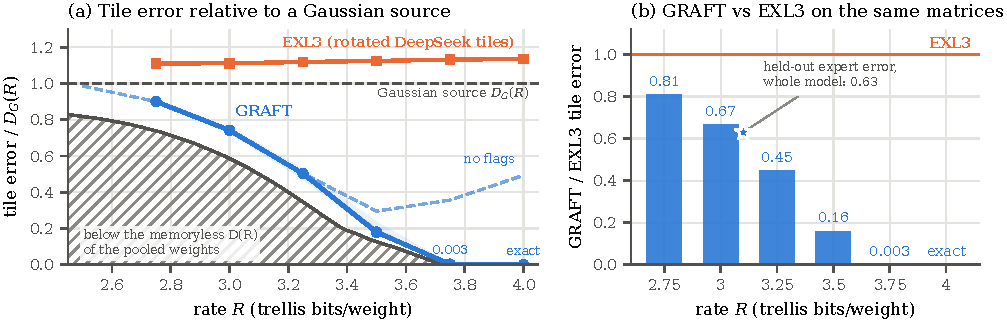
\includegraphics[width=\textwidth]{figures/fig_rd}
\caption{GRAFT's tile error relative to a Gaussian source. (a) Raw-tile error divided by $D_G(R)=2^{-2R}$, the
distortion--rate function of a Gaussian source of the same variance. GRAFT (solid; block flags where they pay for their
bit, per-matrix widths, tail band 0) on every routed-expert matrix of 11 layers of DeepSeek-V4.1-Flash
(\final{MX11-N} matrices, 96 seeded tiles each; median, interquartile and 10--90\% bands) reaches \final{GRAFT-GAUSS3}
at 3 bits, \final{GRAFT-GAUSS35} at 3.5 and \final{GRAFT-GAUSS375} at 3.75, and at 4 bits it reproduces every sampled
tile of \final{EXACT4} of the matrices exactly. Dashed: the same codebook without flags on all 46,080 matrices. It
stops improving above 3.5 bits (\final{NOFLAG-GAUSS4} at 4), because blocks whose MX scale is an octave below their
column's need the halved grid, which only the flags provide. Squares: EXL3's codebook on \final{ROT-N} of these
matrices after EXL3's rotation (\final{ROT-TILES} tiles each, median), at about \final{EXL3-ROT-X} $D_G(R)$; on
Gaussian tiles it comes within \final{EXL3-GAUSS} of $D_G(R)$. Hatched: below the memoryless distortion--rate
function of the pooled weights (entropy \final{DS-ENTROPY} bits), a reference for the per-matrix medians rather than a
bound for each matrix. The rate counts trellis bits only. (b) GRAFT's tile error relative to EXL3's on the same \final{ROT-N} matrices
(median of the per-matrix ratios); star: GRAFT's held-out expert error relative to EXL3 over the whole model at 3
bits.}
\label{fig:rd}
\end{figure*}

\section{GRAFT}
\label{sec:method}

GRAFT is a deterministic post-training quantizer for weights released on an MXFP4 grid. It codes each matrix
$W\in\mathbb{R}^{k\times n}$ ($k$ inputs, $n$ outputs) at 3 bits per weight with a trellis whose decoded values are
MXFP4 blocks, combined with per-column scales (\cref{fig:pipeline}).

\begin{figure}[b!]
\centering
\begin{tikzpicture}[font=\scriptsize, node distance=2.2mm,
  box/.style={draw=black!55, rounded corners=1.5pt, fill=#1, minimum height=6mm, align=center, inner sep=2pt},
  box/.default=white, ar/.style={-{Stealth[length=1.5mm]}, black!60}]
\node[box=blue!6] (state) {16-bit\\state $s$};
\node[box, right=of state] (hash) {$h=$ bytesum\\$(s\cdot\texttt{0x83DCD12D})$};
\node[box=green!7, right=of hash] (map) {$2^{1-f}\,\mathrm{E2M1}\big(\tfrac{h-510}{w_f}\big)$};
\node[box=orange!8, below=3mm of map] (tail) {$|h-510|\le d$:\\$2^{-f}(\pm2^m\{1,1.5\})$};
\node[box, right=of map] (scale) {$\times\,2^{p_j}\alpha_j$};
\draw[ar] (state) -- (hash); \draw[ar] (hash) -- (map); \draw[ar] (map) -- (scale);
\draw[ar] (hash.south) |- (tail.west); \draw[ar] (tail.east) -| (scale.south);
\end{tikzpicture}
\caption{Decoding one weight. The state is the 16-bit window of the bitstream that ends at the current step, and the
hash is EXL3's. GRAFT's value map is the hardware E2M1 conversion, scaled by the flag $f\in\{0,1\}$ of the weight's
32-input block, or, for states at the hash centre, a power-of-two ladder (tail). No inverse rotation is needed.
Outside the tail every block is an MXFP4 block with scale $2^{1-f}$, and the tail values form an exact sparse
correction.}
\label{fig:pipeline}
\end{figure}

\paragraph{Trellis.} GRAFT uses EXL3's 16-bit bitshift trellis, which codes each 16$\times$16 tile in tensor-core
order as one tail-biting ring of 256 steps. At 3 bits per weight the decoder shifts in three bits per step, so a tile
holds 768 bits.

\paragraph{The grid-aligned codebook.} GRAFT keeps EXL3's hash $h(s)$ but replaces the value map. A weight in
row $i$ and column $j$ belongs to the MX block of rows $32\lfloor i/32\rfloor$ to $32\lfloor i/32\rfloor+31$ of
column $j$. If this block has flag $f\in\{0,1\}$ ($f=0$ in a matrix without flags), the weight's trellis state $s$
decodes to
\begin{equation*}
v(s)=2^{-f}\begin{cases}\pm 2^{m}\{1,1.5\} & |h-510|\le d,\\
2\,\mathrm{E2M1}\big(\tfrac{h-510}{w_f}\big) & \text{otherwise},\end{cases}
\end{equation*}
with $h=h(s)$. The bulk value is computed as $\mathrm{E2M1_{RNE}}(\mathrm{fp32}((2^{23}+h)q_a^{(f)}+q_b^{(f)}))$
with $q_a^{(f)}=1/w_f$ and $q_b^{(f)}=-(2^{23}+510)q_a^{(f)}$, which takes one fused multiply-add and the GPU's E2M1
conversion. In an unflagged block the bulk takes the 15 values $\{0,\pm1,\pm2,\pm3,\pm4,\pm6,\pm8,\pm12\}$, and a
flagged block decodes to half these values, $\{0,\pm0.5,\dots,\pm6\}$, with its own width $w_1$. A column normalized
by one power of two contains blocks whose MXFP4 scale is an octave below the column's, and the flag gives these blocks
the grid they need. The width $w_f$ sets how the Gaussian-like hash spreads over the grid. A tail state takes its sign
from bit 0 of $s$ and its magnitude from $\rho=(s\gg1)\bmod 26$ as $2^{3+\lfloor\rho/2\rfloor}$, multiplied by 1.5
if $\rho$ is odd, which gives 26 magnitudes from 8 to $49{,}152$ (\cref{fig:qtail}). Because the bulk map outputs
zero at the hash centre, the band trades a small part of the zero mass for range. It covers
\final{TAIL-D0} states (0.27\%) at $d=0$ and \final{TAIL-D20} (10.7\%) at $d=20$. The fit uses $d=0$ on
\final{BAND0} of the matrices and never more than $d=\final{BANDMAX}$, and \final{BAND-LATE} of the others lie in the
last three layers, where the outliers are.

\paragraph{Decoded representation.} Outside the tail, $v=2^{1-f}e$ with $e$ an E2M1 value, so every (32-input block,
column) pair of a GRAFT matrix decodes to an OCP MXFP4 block, that is, to E2M1 codes with the power-of-two block
scale $2^{1-f}$. The flag is the block's MX scale stored in one bit. The full reconstruction is
$\widehat W=(B+T)\,\mathrm{diag}(c)$, where $B$ holds these MXFP4 blocks, $T$ is the sparse tail and
$c_j=2^{p_j}m_g\alpha_j$ is the column scale. The matrix $B$ is MXFP4, but $\widehat W$ in general is not, because
$\alpha_j$ is a free fp16 factor and tail values lie outside their block's range. Both are applied outside the
block-scaled product. A tail value is an exact FP8 number, which a decoder applies as a sparse correction
next to the block at the cost of one product per tail weight (\final{TAILS} of the weights in our fits). Every decoded value is $0$ or $\pm2^e\{1,1.5\}$, an exact FP8 E5M2 number.

\begin{figure}[t]
\centering
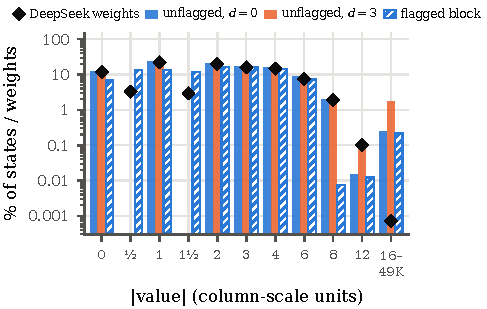
\includegraphics[width=\linewidth]{figures/fig_qtail}
\caption{GRAFT's codebook compared with its source. Bars: share of the 65,536 trellis states that decode to each
magnitude in an unflagged block (width 95.68) at tail band $d=0$ and $d=3$, and in a flagged block (hatched; its own
table at width 53, the most common width in the fit, halved). The last bar pools the tail ladder $2^m\{1,1.5\}$,
$m=3..15$, up to 49,152. Diamonds: share of DeepSeek-V4.1-Flash's routed-expert weights at each magnitude in the same
column units (\final{SRC-N} matrices). On the grid the codebook follows the source, including zero (\final{ZERO-D0}
of the states, \final{SRC-ZERO} of the weights). The halves (\final{SRC-HALF} of the weights) lie in blocks an octave
below their column's MX scale, and a flagged block's table puts \final{FLAGTAB-HALF} of its states on them. To reach
the outliers, which are rare (\final{SRC-TAIL} of these weights lie above 12), the tail takes its states from the hash
centre, where the bulk decodes to zero (\final{ZERO-D3} of the states at $d=3$). The fit uses $d=0$ on \final{BAND0}
of the matrices.}
\label{fig:qtail}
\end{figure}

\paragraph{Scales.} Each column is scaled by $2^{p_j}m_g\alpha_j$. The first factor is a power of two that brings to
3 the RMS of the column's weights that lie within $16\times$ its RMS, so that a few huge weights, which the tail codes,
do not inflate it. The second is a power-of-two multiplier $m_g\in\{1,2,4,8\}$ for densely heavy columns, shared by
each group of 16 columns (one tile wide). The third is an fp16 factor $\alpha_j$, computed in closed form after the fit
as the $H$-weighted least-squares fit of the decoded column. Free (non-power-of-two) scales give \final{FREE-SCALES}
more error.

\paragraph{Parameter selection.} The widths, the tail band $d$, the group multipliers and the flags are all chosen
with one quantity, the \emph{fit-weighted tile error}
\begin{equation*}
E=\sum_{t}\frac{1}{p_t}\sum_{(i,j)\in t} \delta_i s_j\,(\hat w_{ij}-w_{ij})^2 ,
\end{equation*}
which is the error of the trellis when it codes a $16\times16$ tile $t$ on its own (without error feedback) under the
per-weight costs of the fit ($\delta_i$ is the block-LDL diagonal of the shrunk $H$ and $s_j$ the column weight),
summed over 256 tiles drawn with probability $p_t$ proportional to their share of $\sum\delta_i s_j w_{ij}^2$. Without
flags, $(w_0,d)$ is chosen by coordinate descent, and each group's multiplier by the same error over all of the
group's tiles. At those scales we try three flag rules, each with its own widths. The first flags every block for
which rounding its scaled weights onto the halved grid gives the lower fit-weighted error, and the other two flag the
blocks whose largest scaled magnitude is at most 4 or at most 5. A rule with flags is charged a factor of $4^{1/32}$,
which is what its $1/32$ bit per weight is worth on the Gaussian rate curve, and the cheapest of the four options is
fitted. Sampling the tiles by importance under the fit's costs matters, because uniform, unweighted tiles misjudge
matrices whose error concentrates in a few heavy rows.

\paragraph{Objective and encoder.} For each matrix the fit minimizes $\sum_j s_j(w_j-\hat w_j)^\top H(w_j-\hat w_j)$
over its columns $w_j$. In the input-by-output convention, a gated MLP with gate pre-activations $z=W_1^\top x$ and
up activations $u=W_3^\top x$ computes $y=W_2^\top\big(\phi(W_1^\top x)\odot W_3^\top x\big)$ (with the model's
activation clamps). The squared sensitivity of the
expert output to gate channel $j$ at token $t$ is $\sigma^{(1)}_{tj}=(\phi'(z_{tj})u_{tj})^2\|W_2[j,:]\|^2$, and to up
channel $j$ it is $\sigma^{(3)}_{tj}=\phi(z_{tj})^2\|W_2[j,:]\|^2$. We approximate each by the product of a column
weight $s_j\propto\sum_t\sigma_{tj}$, normalized to mean 1, and a token weight $\omega_t=\sum_j\sigma_{tj}$, which
gives $H=\sum_t\omega_t x_tx_t^\top/\sum_t\omega_t$. For the down projection, $H$ comes from the quantized gate/up
activations and $s=1$. We shrink $H$ 25\% toward its diagonal and add 1\% damping. The encoder runs reverse
block-LDL error feedback with a weighted tail-biting Viterbi search over all $2^{16}$ states per 16-row block, in
which each position's flag selects its value table. The path cost weights each position by the block-LDL diagonal and
its column weight, $\delta_i s_j$.

\paragraph{MXFP4 operands.}
\label{sec:operands}
Because $B$ consists of MXFP4 blocks, its product runs on existing block-scaled tensor-core GEMMs. A block-scaled
FP4 or FP8 matrix multiply (W4A4, W4A8) takes the E2M1 codes and the block scales $2^{1-f}$ as they are and applies the
column scale per output channel in the epilogue, and the tail correction is a sparse product added to the result. A
W8A8 kernel sees the same values as exact FP8 numbers. The reference implementation of DeepSeek-V4.1-Flash quantizes
each expert activation to E4M3 with one power-of-two scale per 32 inputs and multiplies it with the MXFP4 weights in a
block-scaled FP4 GEMM. To run a GRAFT matrix on this path, a decoder first converts its trellis to MXFP4 codes and
block scales. The GEMM itself is unchanged, and its result receives the column scale (one FP32 multiply per output)
and the sparse tail product. With the native weights, the same path reproduces the reference bit for bit. In our
evaluation the conversion of each layer's experts happens before the GEMM. This validates numerical compatibility, but
decoding inside the GEMM, which keeps the weights compressed in memory, is not measured here.

\paragraph{Storage.} Each matrix stores the trellis words, a rate code, a codebook code, six fp32 constants
($q_a,q_b$ for each flag state and $d$), the fp16 column scales and, if the matrix uses flags, one bit per 32-input
block and column. This amounts to $3kn+16n+208$ bits, plus $kn/32$ with flags, which gives \final{BPW-NOFLAG} bits per
weight on DeepSeek's experts without flags and \final{X-BPW} on average with them (EXL3 at 3.0 stores
\final{BPW-EXL3}). The code consists of the trellis words alone, with no escapes or side tables.

\section{Experiments}
\label{sec:experiments}

\paragraph{Setup.} We code all 15,360 routed experts (46,080 matrices) of DeepSeek-V4.1-Flash, each at 3 bits per
weight. Calibration uses up to 65,536 routed rows per expert (seed 41) plus every attention-sink row, drawn from a
mixed web, code, math and multilingual corpus. Expert-level error is the NMSE of the expert output against the native
MXFP4 expert on up to 1,024 held-out routed tokens per expert. We aggregate it over the model as the ratio of mean
expert NMSE to EXL3's, with every expert weighted equally, and give the geometric mean of the per-expert ratios in
parentheses. The baseline is EXL3 at 3.0 bits per weight as published (exllamav3's own quantizer, rotation and
Hessian), fitted on the same calibration pool with the same seed and cap and measured on identical held-out rows.
Model-level metrics use 400 held-out 2,048-token windows (all 140 of the WikiText-2 test set and 260 from C4
validation), scored against the native model with llama.cpp's rule, which scores the second half of each window
without BOS (409,200 scored tokens). We report KL divergence, excess NLL of the true next token and top-1 agreement,
with paired bootstrap 95\% intervals over windows.

\paragraph{Damage and divergence.} Our evaluation runs the experts in FP16 arithmetic. With the \emph{native}
weights, this path alone has KL \final{F-KL} to the reference (top-1 \final{F-T1}) at an excess NLL of \final{F-NLL}.
Ulp-level differences swap near-tied top-$k$ routes, and the swaps propagate through later
layers~\citep{fu2025eaquant,park2026vsraq,gu2026routeflip}, but the change in mean NLL on these corpora is negligible.
Because KL also counts such route swaps, we take excess NLL as the measure of damage and KL as a measure of divergence,
and we compare KL only between models in the same arithmetic. GRAFT's decoded weights also run on the
reference's own expert kernels (\cref{sec:operands}). There the native weights reproduce the reference exactly, so
every difference comes from GRAFT's weights.

\begin{table*}[t]
\centering
\caption{DeepSeek-V4.1-Flash at 3 bits per weight (routed experts). Expert: held-out expert NMSE relative to EXL3 on
the same rows, ratio of means (geometric mean of ratios). Model level: 400 windows scored with the llama.cpp rule;
excess NLL of the true next token ($\Delta$NLL, nats), KL divergence and top-1 agreement against the native model,
with the experts in FP16 arithmetic except on the reference kernels. The second row is a control that runs the native
weights through the same FP16 arithmetic. Bits: stored bits per expert weight, all tensors
included.
$^\dagger$Ablation: per-matrix octave codebook instead of block flags (\cref{tab:ablation}).}
\label{tab:main}
\small
\setlength{\tabcolsep}{5pt}
\begin{tabular}{lccccc}
\toprule
 & bits & expert & $\Delta$NLL & KL & top-1\\
\midrule
native MXFP4 & 4.25 & -- & 0 & 0 & 100\%\\
\quad FP16 expert arithmetic & 4.25 & -- & \final{F-NLL} & \final{F-KL} & \final{F-T1}\\
EXL3 & 3.010 & 1.00 & \final{E-NLL} & \final{E-KL} & \final{E-T1}\\
\textbf{GRAFT} & 3.006 & \final{X-MEAN} (\final{X-GEO}) & \final{G-NLL} & \final{G-KL} & \final{G-T1}\\
\quad reference kernels & 3.006 & & \final{R-NLL} & \final{R-KL} & \final{R-T1}\\
octave codebook$^\dagger$ & 3.004 & \final{O-MEAN} (\final{O-GEO}) & \final{O-NLL} & \final{O-KL} & \final{O-T1}\\
\bottomrule
\end{tabular}
\end{table*}

\paragraph{Expert level.} Over the whole model, GRAFT's mean held-out expert error is \final{X-MEAN}$\times$ that of
EXL3 (geometric mean of the per-expert ratios \final{X-GEO}$\times$), and its error is lower on all but
\final{X-WORSE} of the \final{X-N} experts with held-out rows. The ratio is flat across depth (\final{X-LAYERS} per
layer; \cref{fig:layers}a). This is what the discrete-source argument predicts for a source whose grid structure is
the same in every layer. At 3 bits the memoryless reference is about \final{DS-BOUND3-1}$\times$ $D_G$, and GRAFT's
tile error is about \final{GRAFT-BOUND3} that reference. On tiles (\cref{fig:rd}b), where EXL3's codebook codes the
same \final{ROT-N} DeepSeek matrices after EXL3's rotation, the median over matrices of GRAFT's error relative to
EXL3's is \final{TILE-275} at 2.75 bits, \final{TILE-3} at 3, \final{TILE-325} at 3.25, \final{TILE-35} at 3.5 and \final{TILE-375} at 3.75.
The advantage thus grows with the rate, and at 4 bits GRAFT reproduces every sampled tile of \final{EXACT4} of the
matrices exactly.

\paragraph{Model level.} GRAFT's excess NLL is \final{G-NLL} nats against \final{E-NLL} for EXL3, a ratio of
\final{G-NLLR} (paired difference \final{G-DNLL-X}). Its KL is \final{G-KL} against \final{E-KL}, a ratio of
\final{G-KLR} (paired difference \final{G-DKL-X}), and its top-1 agreement is \final{G-T1} against \final{E-T1}. On
the reference's own kernels, GRAFT's KL is \final{R-KL}, slightly above that of the FP16 path (paired difference
\final{R-DKL-G}), and its excess NLL is \final{R-NLL}. Removing the arithmetic's own perturbation therefore does not
lower GRAFT's KL. This is consistent with the route swaps caused by the arithmetic overlapping those caused by the
weights rather than adding to them, although we did not trace individual routes to confirm the mechanism. Either
way, KL measured in one arithmetic cannot be split into an arithmetic part and a weight part by subtraction.

\begin{figure*}[t]
\centering
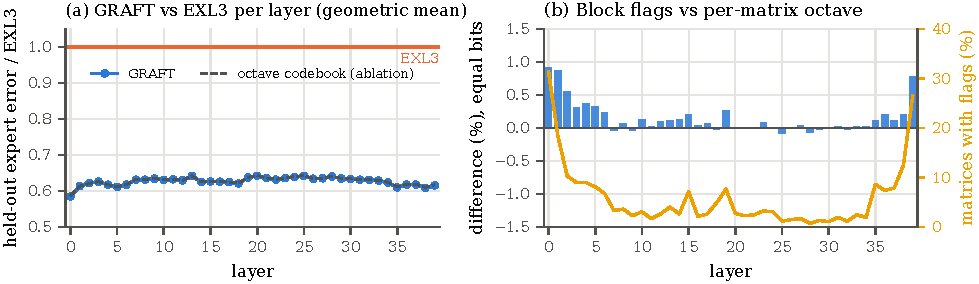
\includegraphics[width=\textwidth]{figures/fig_layers}
\caption{Held-out expert error per layer on DeepSeek-V4.1-Flash at 3 bits. (a) GRAFT and the octave-codebook ablation
relative to EXL3 on the same rows (geometric means; the two curves overlap). (b) Difference between GRAFT's error and
the octave codebook's at equal bits (bars), $100(\text{GRAFT}/\text{octave}-1)$, where zero means equal error, and
the share of matrices whose fit uses block flags (line).}
\label{fig:layers}
\end{figure*}

\paragraph{Ablations.} \Cref{tab:ablation} quantifies GRAFT's design choices. Every row is fitted on the same
calibration rows and measured on the same held-out rows. Where an ablation spends a different number of bits, we
compare at equal bits using the measured held-out rate curve of the octave-codebook fit, which gives an error factor
of \final{RHO} per extra quarter bit at 3 bits (14 experts).
\begin{itemize}[leftmargin=1.1em,itemsep=1pt,topsep=2pt]
\item \emph{The code or the fitting objective.} GRAFT's fit differs from EXL3's in the objective (gated,
token-weighted $H$ and column weights, shrinkage, down-projection statistics from the quantized gate/up activations)
as well as in the code. An EXL3 refit with GRAFT's objective on the same calibration rows has \final{ATTR-OBJ} the
held-out error of EXL3 as published (geometric mean \final{ATTR-OBJ-GEO}, \final{ATTR-N} experts). GRAFT has
\final{ATTR-G} the error of this refit (geometric mean \final{ATTR-G-GEO}) and is lower on all but
\final{ATTR-G-WORSE} experts, so the objective accounts for a few percent and the grid-aligned code for the rest.
\item \emph{Block flags or a per-matrix octave codebook.} Instead of using flags, a matrix can move a fraction of its
trellis states one octave down, so that states whose top bits are set decode at half value. The two approaches reach
the same error. Over all \final{X-N} experts, the octave codebook has \final{O-RAW} GRAFT's held-out error at GRAFT's
bits and \final{O-EQ} at equal bits. The two are within $\pm$0.3\% in \final{O-LAYERS-N} of
40 layers and at most \final{O-LAYERS-MAX} apart in the first and last layers (\cref{fig:layers}b). The model-level KL
of the octave codebook is \final{O-KL}, against \final{G-KL} for GRAFT (difference \final{G-DKL-O}). Flags are needed
on \final{FLAG-SHARE} of the matrices and the octave on \final{OCT-SHARE}, and only flags keep the decoded blocks
MXFP4. On fit tiles at 3.5 bits the flags are ahead, with \final{FLAGS35} the octave codebook's error on
\final{FLAGS35-N} matrices.
\item \emph{Flags off.} On the \final{FLAGSOFF-N} flagged experts of the last layer, removing the flags raises
held-out error by only \final{FLAGSOFF-PCT} at equal bits, so at 3 bits the flags roughly break even on error. Their
benefit is that they keep the decoded blocks MXFP4. They also decode in fewer instructions than
the octave codebook (\final{K-B200-ON} against \final{K-B200-OCT} per weight on B200), and at 3.5 bits they are ahead
(above).
\item \emph{Rate allocation.} Moving bits between matrices according to their predicted contribution to expert
error, at the same stored size, lowers mean expert error by \final{ALLOC-ERR} (octave codebook, all experts) but KL
by only \final{ALLOC-KL}. It also lowers top-1 agreement (\final{ALLOC-T1} vs \final{FLAT-T1}) and raises excess NLL
(\final{ALLOC-NLL} vs \final{FLAT-NLL} on 40 windows, too few to resolve the difference). Allocation by our
expert-error estimator therefore did not improve model-level quality in this experiment, and GRAFT codes every
matrix at the same rate.
\item \emph{The trellis or a 3-bit scalar code.} Scalar 3-bit codebooks of 8 values per 8 columns, fitted with the
same objective and error feedback, have \final{SCALAR-EF} GRAFT's held-out error at the same bits (\final{SCALAR-N}
experts in \final{SCALAR-LAYERS} layers). With plain rounding they have \final{SCALAR-RTN}, and with an MX block
scale per 32 weights at \final{SCALAR-MX-BPW} bits they still have \final{SCALAR-MX}. An 8-value table can hold at
most 8 of the source's 15 levels, whereas the fitted trellis reproduces about \final{EXACT} of the source weights
exactly (within 5\% of a grid step after the column scale, on octave-codebook fits of 20 experts at 3 bits).
\end{itemize}

\begin{table}[t]
\centering
\caption{Ablations: error relative to GRAFT (equal bits unless marked). Top: measured held-out expert error on the
experts listed. Bottom: predictions of the selection estimator, not held-out measurements, given as the typical
(geometric-mean) and total fit-weighted tile error of the octave-codebook fits over \final{KNOB-N} matrices.}
\label{tab:ablation}
\footnotesize
\setlength{\tabcolsep}{2pt}
\begin{tabular}{@{}llr@{}}
\toprule
change & measured on & error\\
\midrule
EXL3 code, GRAFT's objective & all experts & \final{ATTR-INV}\\
octave codebook instead of flags & all experts & \final{O-EQ}\\
no block flags & \final{FLAGSOFF-N} experts, L39 & \final{FLAGSOFF}\\
3-bit scalar tables, error feedback & \final{SCALAR-N} experts & \final{SCALAR-EF}\\
\quad plain rounding & \final{SCALAR-N} experts & \final{SCALAR-RTN}\\
\quad + MX scales (\final{SCALAR-MX-BPW} bits) & \final{SCALAR-N} experts & \final{SCALAR-MX}\\
free (non-pow.-two) column scales & earlier code, 2 layers & $+$\final{FREE-SCALES}\\
\midrule
tail band fixed at $d=0$ & estimator & \final{KNOB-BAND-GEO} / \final{KNOB-BAND-TOT}\\
no group multipliers & estimator & \final{KNOB-MULT-GEO} / \final{KNOB-MULT-TOT}\\
\bottomrule
\end{tabular}
\end{table}

\section{Related work}
\label{sec:related}

\paragraph{Compressing low-precision releases.} We know of no method that compresses an FP4-native checkpoint below 4
bits per weight by exploiting its grid. Tied Trit-Planes~\citep{grella2026trit} requantizes DeepSeek-V4-Flash's MXFP4
experts to about 4 bits and treats the dequantized weights as continuous. ReQuant~\citep{requant2026} refines codes on
a fixed grid without lowering the bit width, and \citet{zhao2025deepseek} requantize FP8 DeepSeek releases to
3--4-bit GGUF types. Lossless compression gains almost nothing on MXFP4 and NVFP4 codes~\citep{heilper2025lossless},
which is consistent with our entropy measurements.

\paragraph{Trellis and vector quantization.} GRAFT builds on QTIP's bitshift trellis with computed
codebooks~\citep{tseng2024qtip} as implemented in EXL3~\citep{exllamav3}, on LDLQ and incoherence
processing~\citep{chee2023quip,tseng2024quipsharp}, and on GPTQ-style error
feedback~\citep{frantar2022obc,frantar2023gptq}. Vector and additive
codebooks~\citep{egiazarian2024aqlm,vanbaalen2024gptvq,liu2024vptq,malinovskii2024pvtuning}, Hadamard rotation with
Gaussian-optimal grids~\citep{higgs2025} and fractional-bit allocation for Gaussianized weights~\citep{qpalette2025}
all assume a continuous source. Lattice VQ collapses without rotation on BF16 models~\citep{llvq2026}, which is why a
result without rotation is specific to sources already on a grid. Grid-aligned trellis quantizers exist for
uniform integer grids, including classical TCQ~\citep{marcellin1990tcq}, the dependent quantization of the NNR
standard~\citep{nnr2022} and CCQ~\citep{ccq2025}. XOR-Trellis~\citep{que2026xortrellis} quantizes BF16 checkpoints
using a trellis that decodes to FP4 values with E5M3 group scales. Work on FP4 formats finds that rotations interact
badly with block scales~\citep{egiazarian2025mrgptq,shao2025blockrot,jokar2026inversion}.

\paragraph{Objectives, outliers and allocation.} GRAFT's gated objective is the special case of
Kronecker-factored Hessians~\citep{fastkron2026} with a per-expert, one-sided, diagonal output factor. Such a factor
cancels in plain GPTQ~\citep{kronq2026}, whereas GRAFT applies it through the trellis cost. Outliers are usually
stored exactly beside the code~\citep{dettmers2023spqr,kim2023squeezellm,owq2024,icquant}. GRAFT instead gives the
codebook itself a power-of-two range, which a grid-aligned code can afford because large MXFP4 weights are themselves
powers of two times E2M1 values, and the stored code stays one bitstream. Sensitivity-driven mixed-precision
allocation~\citep{dong2019hawq,higgs2025} is orthogonal to the code. In our experiment on this model, moving bits between
experts according to our expert-error estimates did not improve model-level quality (\cref{sec:experiments}).

\section{Limitations and conclusion}
\label{sec:conclusion}

\paragraph{Limitations.} We report results for one model; results on gpt-oss~\citep{gptoss} are coming soon. We
evaluate GRAFT at 3 bits per weight. Its tile-level advantage grows with the rate (\cref{fig:rd}), but we do not
evaluate higher rates end to end here. Model-level metrics use 400 windows from two text corpora, and we do not report
capability benchmarks. We do not measure throughput or latency, and the reference-kernel evaluation decodes each
layer's experts to MXFP4 operands before the matrix multiply.

\paragraph{Decode cost and speed.} Like EXL3 and QTIP~\citep{exllamav3,tseng2024qtip}, GRAFT decodes on the
general-purpose cores rather than on the tensor cores. For each weight, the decoder extracts the 16-bit state (a shift
and a mask), computes the hash (an integer multiply and a byte-sum dot product) and applies the value map (a fused
multiply-add and half an FP4 conversion). On Blackwell (B200) this takes about \final{K-B200-OFF} instructions in an
unflagged block and \final{K-B200-ON} with a flag, against \final{K-B200-OCT} for the per-matrix octave codebook.
The smaller representation reduces weight traffic, but whether this decode work is hidden and the saving turns into
throughput depends on overlapping the decode with memory access. Where decode itself sets the speed, as on HBM GPUs such as B200, a throughput model puts GRAFT's expert
products at an estimated 2--3$\times$ the time of native MXFP4, so on these GPUs its benefit is capacity. The decode
cost cannot be traded away cheaply. On \final{DEC-N} DeepSeek matrices (\final{DEC-HI-N} for the bit-sliced
decoders), every cheaper state-to-value map we screened (top-bit and register tables, two weights per state, linear and
bit-sliced decoders) raised weight error by \final{DEC-RANGE}, whereas a random permutation of GRAFT's own table raised
it by \final{DEC-PERM}. The byte-sum hash spreads the successors of a state better than random draws do. Hardware support
for trellis decoding in the tensor-core operand path, like today's support for 2:4 sparsity metadata and MX block
scales~\citep{rouhani2023mx}, would remove this cost for EXL3 and QTIP as well as for GRAFT.

\paragraph{Conclusion.} An MXFP4 checkpoint is a discrete source, and a quantizer that keeps the grid instead of
rotating it away can go well below the Gaussian-source curve for which rotation-based, Gaussian-matched coders are
designed. GRAFT does this inside EXL3's
trellis by changing only the value map. The new map applies an E2M1 conversion to EXL3's hash, with a one-bit MX
scale per block and a power-of-two tail at the hash centre, so the bulk decodes to MXFP4 blocks again. On
DeepSeek-V4.1-Flash, GRAFT has \final{X-MEAN2}$\times$ EXL3's held-out expert error at 3 bits, and its MXFP4 blocks
run on the model's own MXFP4 kernels with a per-column output scale and a sparse tail correction added. GRAFT
therefore stores the experts in fewer than 4 bits per weight while the bulk of the computation stays in the format the
model was trained in.


\bibliographystyle{plainnat}
\bibliography{refs}

\end{document}
